\section{Structured Masked Attention: Generalizing Linear Attention \texorpdfstring{\\}{} with Structured Matrices}
\label{sec:attention}

%



In this section we revisit the linear attention framework from first principles.
The main results in this section are a simple tensor-contraction-based proof of linear attention (\cref{prop:linear-attention}),
and our generalized abstraction of structured masked attention in \cref{def:sma}.
\iftoggle{arxiv}{
We note that this section derives the main duality results from a different direction than state space models and can be read completely independently of \cref{sec:ssm}.
}{}

\begin{itemize}
  \item \cref{sec:masked-attention} sets up our framework for variants of attention, with a particular focus on kernel attention and masked kernel attention.
  \item \cref{sec:linear-attention} provides our first main attention result, a simple proof of linear attention through the lens of tensor contractions.
  \item \cref{sec:structured-attention} defines structured masked attention, our generalization of prior attention variants through structured matrices.
\end{itemize}

\subsection{The Attention Framework}
\label{sec:masked-attention}

\subsubsection{Attention}
The basic form of (single-head) attention is a map on three sequences of vectors $(Q, K, V) \mapsto Y$.
\begin{equation}
  \label{eq:kernel-attention}
  \begin{aligned}%
    Q &= \mathsf{input} & \mathtt{(T,N)} \\
    K &= \mathsf{input} & \mathtt{(S,N)} \\
    V &= \mathsf{input} & \mathtt{(S,P)} \\
    G &= QK^\top        & \mathtt{(T,S)} \\
    M &= f(G)           & \mathtt{(T,S)} \\
    Y &= GV             & \mathtt{(T,P)} \\
  \end{aligned}
\end{equation}
We use ``shape annotations'' to indicate the dimensions of tensors, e.g.\ $Q \in \R^{\mathtt{(T,N)}}$.
In this general form, $\mathtt{S}$ and $\mathtt{T}$ represent \emph{source} and \emph{target} sequence lengths,
$\mathtt{N}$ represents the \emph{feature dimension}, and $\mathtt{P}$ represents the \emph{head dimension}.

The most common variant of \textbf{softmax attention} uses a softmax activation $f=\mathsf{softmax}$ to normalize the rows of the $G$ matrix.

\subsubsection{Self-Attention}
Our treatment is motivated by the most important case of self-attention, where
\begin{enumerate}[label=(\roman*)]
  \item the source and target sequences are the same (i.e.\ $\mathtt{S}=\mathtt{T}$),
  \item usually the feature and head dimensions are the same (i.e.\ $\mathtt{N}=\mathtt{P}$),
  \item and $Q, K, V$ are generated by linear projections on the same input vector ($Q = W_Q \cdot X, K = W_K \cdot X, V = W_V \cdot X$).
\end{enumerate}
However, our presentation abstracts away these choices and begins from the $Q, K, V$ matrices.

\begin{remark}
  Our focus is on the self-attention case with equal head and feature dimensions (i.e.\ $\mathtt{S}=\mathtt{T}$ and $\mathtt{N}=\mathtt{P}$),
  which should be used as the running example.
  We define the general formulation of attention not only so that our framework captures variants such as cross-attention,
  but also because separating the notation for dimensions (e.g.\ $\mathtt{S}$ and $\mathtt{T}$) makes the contraction notation proofs
  of our main results in this section more clear.
\end{remark}

\begin{remark}
  \label{rmk:attention-input}
  While attention is usually framed as an operation on these three inputs $Q, K, V$ which are viewed symmetrically,
  the input and output dimensions in \eqref{eq:kernel-attention} indicate otherwise.
  In particular, the feature dimension $\mathtt{N}$ is not present in the output;
  therefore in the case when $\mathtt{S}=\mathtt{T}$ (e.g.\ self-attention),
  we view $V$ as the main input, so that \eqref{eq:kernel-attention} defines a proper sequence transformation $V \mapsto Y$ (\cref{def:sequence-transformation}).
\end{remark}

\subsubsection{Kernel Attention}
\label{sec:attention:kernel}

The step where the softmax function is applied to the Gram matrix $G$ can be decomposed into two parts:
\begin{enumerate}
  \item Exponentiating the $G$ matrix.
  \item Normalizing the $G$ matrix on the $\mathtt{S}$ axis.
\end{enumerate}
We can ignore the normalization term for now, as it amounts to simply passing in $V=1$ and dividing\iftoggle{arxiv}{ (we revisit this in \cref{sec:architecture:kernels})}{}.
The exponentiation term can be viewed as a kernel transformation:
there is an (infinite-dimensional) feature map $\varphi$ such that $\exp(QK^{\top}) = \varphi(Q)\varphi(K)^{\top}$.
By abstracting away the feature map into the definition of $Q$ and $K$ itself (i.e.\ define $Q, K$ as the post-transformed versions),
we can ignore the softmax transformation, and assume that $Q, K$ are arbitrarily generated by kernel feature maps and potentially $\mathtt{N} \neq \mathtt{P}$.

Many instantiations of kernel attention have been proposed, including:
\begin{itemize}
  \item The original Linear Attention \citep{katharopoulos2020transformers} defines the kernel feature map as an arbitrary pointwise activation function, such as $x \mapsto 1+\mathsf{elu}(x)$.
  \item Random Feature Attention (RFA)~\citep{peng2021random} chooses the kernel feature map to approximate softmax attention (i.e. the $\exp$ feature map) using the random Fourier feature approximation of Gaussian kernels~\citep{rahimi2007random}. This involves random projections (i.e.\ multiplying $Q$ and $K$ by a random projection $W$ and applying the activation $x \mapsto (\cos(x), \sin(x))$.
%
  \item Performer~\citep{choromanski2021rethinking} proposes the fast attention via positive orthogonal random features (FAVOR+).
    The positive random features (PRF) part chooses the kernel feature map to be a random projection followed by the feature map $x \mapsto 2^{-1/2}(\exp(x), \exp(-x))$.
    This choice is motivated so that the kernel elements are positive-valued and provably approximates the softmax attention. [It also proposes choosing the random projections in orthogonal directions, which we do not consider.]
  \item cosFormer~\citep{qin2022cosformer} augment RFA with a cosine reweighting mechanism that incorporates positional information to emphasize locality.
    This effectively passes $Q_t,K_t$ through the feature map $x \mapsto (x \cos(\pi t / 2T), \sin(\pi t / 2T))$.
  \item Linear Randomized Attention~\citep{zheng2022linear} generalize RFA from the perspective of importance sampling, and generalize it to provide better estimates of the full softmax kernel (rather than just the $\exp$-transformed numerator).
\end{itemize}

Other related attention variants include Linformer~\citep{wang2020linformer} and Nystr\"{o}former~\citep{xiong2021nystromformer}, which both use low-rank approximations of the attention matrix $M$ (and are thus compatible with equation \eqref{eq:kernel-attention}), through random projections (Johnson-Lindenstrauss) and kernel approximation (the Nystr\"{o}m method) respectively.


\subsubsection{Masked (Kernel) Attention}

%

Let $L$ be a mask of shape $\mathtt{(T,S)}$.
Most commonly, in the \emph{autoregressive} self-attention case when $\mathtt{S}=\mathtt{T}$,
$L$ may be a lower-triangular matrix of $1$'s representing a \emph{causal mask}.
Besides enforcing causality, many other types of masks can be applied -- in particular various sparsity patterns such as banded, dilated, or block diagonal -- which are motivated by reducing the complexity of dense attention. %

Masked attention is usually written in matrix notation as
\begin{equation}%
  \label{eq:sha-quad-matrix}
  y = (L \circ (QK^\top)) \cdot V
  .
\end{equation}
More precisely, with shape annotations and breaking this down into the precise sequence of computations:
\begin{equation}
  \label{eq:sha-quad-0}
  \begin{aligned}%
    G &= QK^\top & \mathtt{(T,S)} \\
    M &= G \circ L & \mathtt{(T,S)} \\
    Y &= M V & \mathtt{(T,P)}
  \end{aligned}
\end{equation}

Our improved derivation of attention variants in this section starts by noticing that this formula can be written as a \emph{single contraction}:
\begin{equation}
  \label{eq:sha}
  Y = \mathsf{contract}(\mathtt{TN},\mathtt{SN},\mathtt{SP},\mathtt{TS} \to \mathtt{TP})(Q, K, V, L)
\end{equation}

and the algorithm in \eqref{eq:sha-quad-0} can be reframed as computing \eqref{eq:sha} by a particular ordering of pairwise contractions
\begin{subequations}
  \label{eq:sha-quad}
  \begin{align}%
    \label{eq:sha-quad:1}
    G &= \mathsf{contract}(\mathtt{TN, SN} \to \mathtt{TS})(Q, K) && \qquad \mathtt{(T,S)} \\
    \label{eq:sha-quad:2}
    M &= \mathsf{contract}(\mathtt{TS, TS} \to \mathtt{TS})(G, L) && \qquad \mathtt{(T,S)} \\
    \label{eq:sha-quad:3}
    Y &= \mathsf{contract}(\mathtt{TS, SP} \to \mathtt{TP})(M, V) && \qquad \mathtt{(T,P)}
  \end{align}
\end{subequations}

\subsection{Linear Attention}
\label{sec:linear-attention}

Linear attention, and many other variants of efficient attention, is often motivated by changing the order of matrix associativity in the core attention computation $(QK^\top)V = Q(K^\top V)$.
However when the mask is added, the derivation is somewhat less straightforward (for example, the original paper~\citep{katharopoulos2020transformers} and variants~\citep{sun2023retentive} state the formula without proof).

Roughly, the linear attention method claims that the following formula
is equivalent to \eqref{eq:sha-quad-matrix}, which must be verified by expanding the sum and tracking indices carefully.
\begin{equation}
  \label{eq:sha-lin-matrix}
  Y = Q \cdot \mathsf{cumsum}(K^\top V)
\end{equation}

\begin{proposition}[\citep{katharopoulos2020transformers}]
  \label{prop:linear-attention}
  Autoregressive kernel attention, i.e.\ masked kernel attention with the causal mask, can be computed in $O(T)$ time by a recurrence taking constant time per step.
\end{proposition}

\subsubsection{A Tensor Contraction Proof of Linear Attention}

We present a simple and rigorous derivation of linear attention that will also immediately reveal how to generalize it.
The main idea is to perform the contraction \eqref{eq:sha} in an alternate order.
We avoid ambiguous matrix notation and work directly with contraction notation:
\begin{subequations}
  \label{eq:sha-lin}
  \begin{align}
    \label{eq:sha-lin:1}
    Z &= \mathsf{contract}(\mathtt{SP},\mathtt{SN} \to \mathtt{SPN})(V, K) & \mathtt{(S,P,N)} \\
    \label{eq:sha-lin:2}
    H &= \mathsf{contract}(\mathtt{TS},\mathtt{SPN} \to \mathtt{TPN})(L, Z) & \mathtt{(T,P,N)} \\
    \label{eq:sha-lin:3}
    Y &= \mathsf{contract}(\mathtt{TN},\mathtt{TPN} \to \mathtt{TP})(Q, H) & \mathtt{(T,P)}
  \end{align}
\end{subequations}

Intuitively, we interpret this contraction order as follows.

The first step \eqref{eq:sha-lin:1} performs an ``expansion'' into more features, by a factor of the feature dimension $\mathtt{N}$.
The third step \eqref{eq:sha-lin:3} contracts the expanded feature dimension away.
If $K$ is viewed as the input (\cref{rmk:attention-input}),
then $V$ and $Q$ perform the expansion and contraction, respectively.

The second step is the most critical, and explains the \emph{linear} part of linear attention.
First notice that \eqref{eq:sha-lin:2} is just a direct matrix multiplication by $L$ (since the $\mathtt{(P,N)}$ axes can be flattened).
Also note that this is the only term that involves both $\mathtt{T}$ and $\mathtt{S}$ axes,
hence should have $\Omega(\mathtt{TS})$ complexity (i.e.\ quadratic in sequence length).
However, when the mask $L$ is the standard causal attention mask (lower triangular $1$'s),
matrix-vector multiplication by $L$ is identical to a feature-wise cumulative sum
\begin{align*}%
  y = \begin{bmatrix} 1 \\ \vdots & \ddots \\ 1 & \dots & 1 \end{bmatrix} x
  \quad\iff\quad
  \begin{aligned}
    y_0 &= x_0 \\
    y_t &= y_{t-1} + x_t
  \end{aligned}
  .
\end{align*}


%

\subsection{Structured Masked Attention}
\label{sec:structured-attention}

With the tensor contraction perspective of masked attention \eqref{eq:sha-lin},
we can immediately see that the crux of the original linear attention is the fact that \emph{matrix-vector multiplication by the causal mask is equivalent to the cumulative sum operator}.

However, we observe that there is no reason the attention mask has to be all $1$'s.
All that is necessary for linear attention to be fast is for $L$ to be a \emph{structured matrix},
which by definition are those that have fast matrix multiplication\iftoggle{arxiv}{ (\cref{sec:overview:structured-matrix})}{}.
In particular, we can use \emph{any mask matrix} $L$ that has sub-quadratic (ideally linear) matrix-vector multiplication,
which would have the same complexity as standard linear attention by speeding up the bottleneck equation \eqref{eq:sha-lin:2}.

\begin{definition}%
  \label{def:sma}
  \textbf{Structured masked attention (SMA)} (or \textbf{structured attention} for short) is defined as a \emph{function} on queries/keys/values $Q, K, V$ as well as any \emph{structured matrix} $L$ (i.e.\ has sub-quadratic matrix multiplication), through the 4-way tensor contraction
  \begin{align*}
    Y = \mathsf{contract}(\mathtt{TN},\mathtt{SN},\mathtt{SP},\mathtt{TS} \to \mathtt{TP})(Q, K, V, L)
    .
  \end{align*}
  The SMA \textbf{quadratic mode algorithm} is the sequence of pairwise contractions defined by \eqref{eq:sha-quad},
  which corresponds to the standard (masked) attention computation.

  The SMA \textbf{linear mode algorithm} is the sequence of pairwise contractions defined by \eqref{eq:sha-lin},
  where step \eqref{eq:sha-lin:2} is optimized through the subquadratic structured matrix multiplication.
\end{definition}
We can instantiate structured masked attention to any given class of matrix structure.
Some examples include (\cref{fig:sma}):
\begin{itemize}
  \item Linear attention uses a causal mask.
  \item RetNet~\citep{sun2023retentive} uses a decay mask $L_{ij} = \gamma^{i-j} \cdot \mathbb{I}[j \ge i]$ for some decay factor $\gamma \in [0, 1]$.
  \item The decay mask could be generalized to a Toeplitz matrix $L_{ij} = \alpha_{i-j}$ for some learnable (or input-dependent) set of parameters $\alpha \in \mathbb{R}^\mathtt{T}$. This can be interpreted as a form of relative positional encoding, reminiscent of other methods such as AliBi~\citep{press2022train} but multiplicative instead of additive.
  \item Another variant could use a Fourier matrix $L_{ij} = \omega^{ij / \mathtt{T}}$ to encode positional structure a different way.
\end{itemize}
In \cref{sec:ssd}, we consider semiseparable SMA, which defines our main SSD model.

\iftoggle{arxiv}{
\begin{figure}[!t]
  \centering
  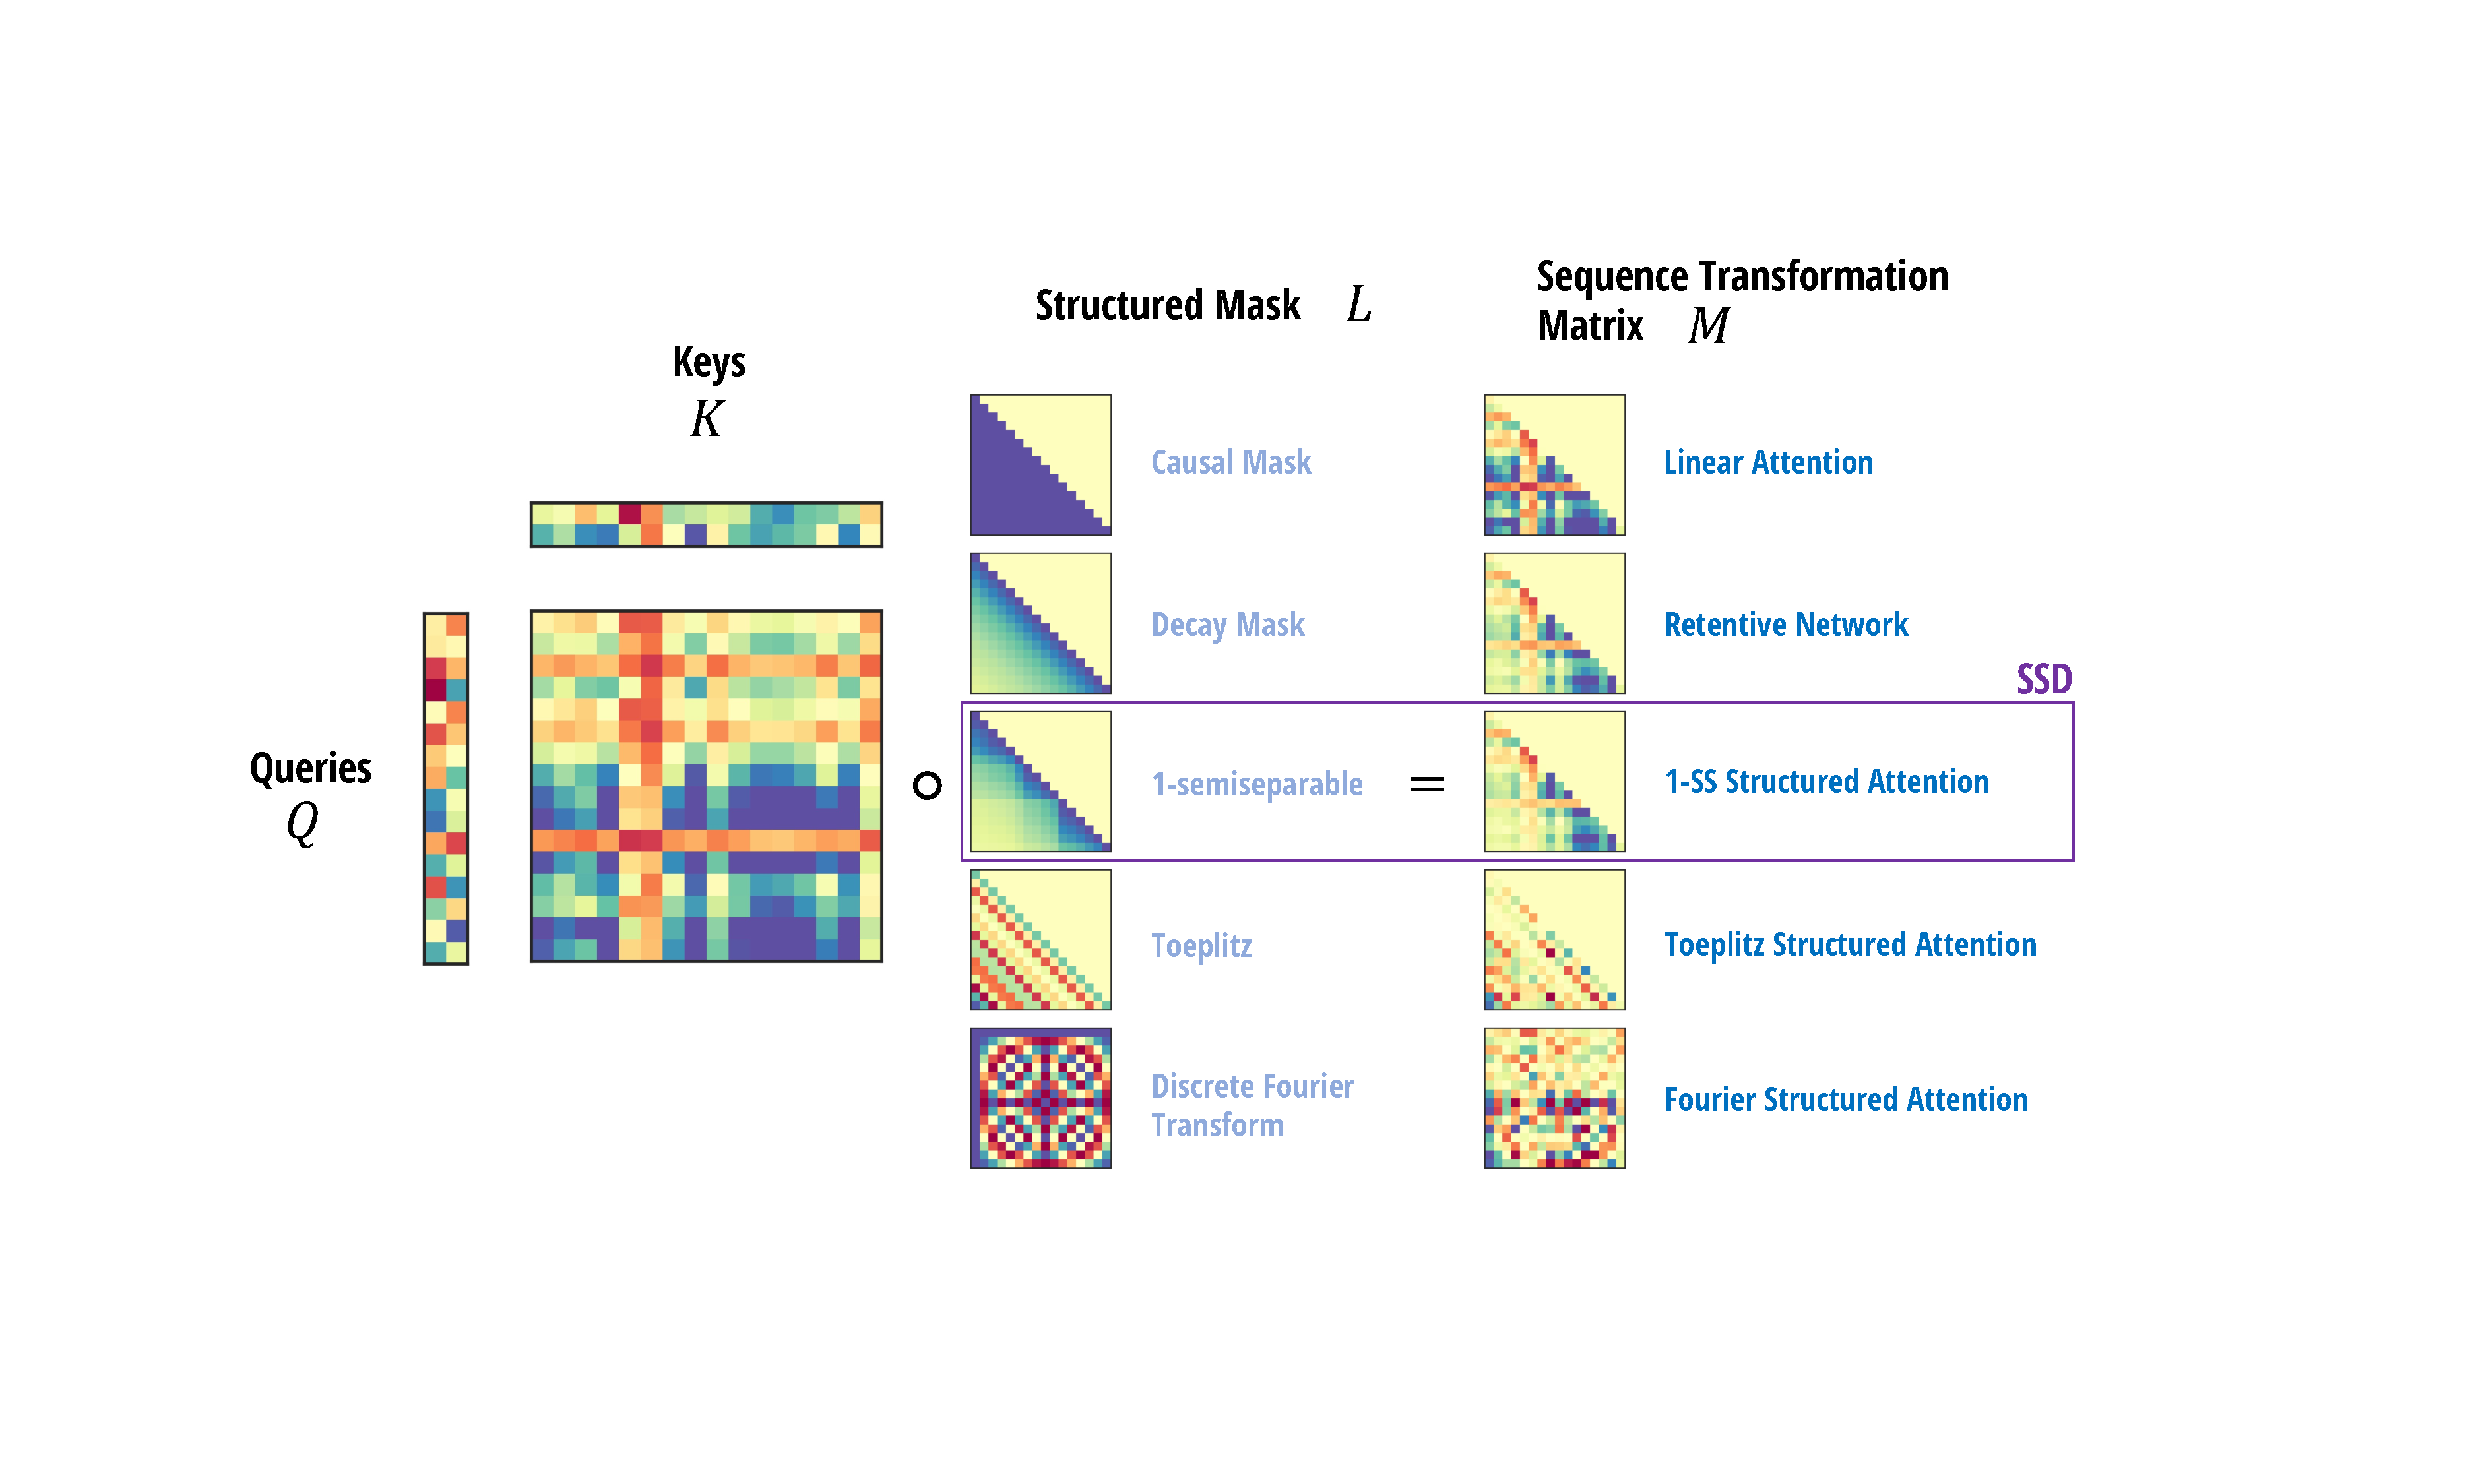
\includegraphics[width=0.9\linewidth]{fig/sma.pdf}
  \caption{
    (\textbf{Structured Masked Attention}.)
    SMA constructs a masked attention matrix $M = QK^\top \circ L$ for any structured matrix $L$, which defines a matrix sequence transformation $Y = MV$.
    All instances of SMA have a dual subquadratic form induced by a different contraction ordering, combined with the efficient structured matrix multiplication by $L$.
    Previous examples include Linear Attention~\citep{katharopoulos2020transformers} and RetNet~\citep{sun2023retentive}.
    Beyond SSD (1-semiseparable SMA), the focus of this paper, many other potential instantiations of structured attention are possible.
  }
  \label{fig:sma}
\end{figure}
}{}


\subsubsection{Summary: The Dual Forms of Masked Attention}

Standard (masked kernel) attention is often conflated between a function and an algorithm.
Separating this distinction presents a clear way to understand different variants of attention.
\begin{itemize}
  \item We view \textbf{masked attention} as a particular \emph{function}~\eqref{eq:sha}.
  \item The standard \textbf{quadratic attention} computation \eqref{eq:sha-quad} can be viewed as an \emph{algorithm} to compute the function.
  \item \textbf{Linear attention} \eqref{eq:sha-lin} is an alternate algorithm to compute the same function.
\end{itemize}

Moreover, in this case
\begin{itemize}
  \item The masked attention function is simply a particular \emph{contraction on four terms}.
  \item The quadratic and linear attention algorithms are simply \emph{two different orders to perform the contractions}.
\end{itemize}
It is known that contraction orderings can make large differences in computation complexity, leading to the quadratic vs.\ linear split.
Just as state space models are a transformation that can be computed in multiple ways, with dual quadratic vs.\ linear forms (\cref{sec:ssm:algorithms}),
linear attention has a similar duality that results from two contraction orders.
\iftoggle{arxiv}{
In fact, these turn out to be different perspectives on the same underlying duality, which we make explicit in \cref{sec:ssd}.
}{}

